\documentclass[conference]{IEEEtran}
\IEEEoverridecommandlockouts
\usepackage{fontspec}
\setmainfont{texgyretermes}[Extension=.otf,UprightFont=*-regular,BoldFont=*-bold,ItalicFont=*-italic,BoldItalicFont=*-bolditalic]
\usepackage{cite}
\usepackage{placeins}
\usepackage{balance}
\usepackage{amsmath,amssymb}
\usepackage{graphicx}
\usepackage{booktabs}
\usepackage{xcolor}
\usepackage{tikz}
\usetikzlibrary{positioning,arrows.meta,fit,backgrounds,calc,shapes.geometric}
\usepackage[hidelinks]{hyperref}
\graphicspath{{figures/}}


\begin{document}

\title{SentriMail: A Human-in-the-Loop Complaint Management System with Multilingual Intake, Hybrid Prioritisation and Compact On-Premise Language-Model Assistance}

\author{\IEEEauthorblockN{Naveen Kumar N, Lohith M, Vansh Paryani, Yash Kumar and Prof.\ Syeeda Mujeebunnisa}
\IEEEauthorblockA{\textit{Department of Artificial Intelligence and Machine Learning}\\
\textit{BMS College of Engineering}, Bengaluru, India\\
\{naveenkumarn.ai24, lohithm.ai24, vanshparyani.ai23, yashkumar.ai23, syeedamujnaseeba.mel\}@bmsce.ac.in}}

\maketitle

\begin{abstract}
Small organisations handle customer complaints through shared mailboxes and spreadsheets: messages arrive in several languages, urgent cases wait behind trivial ones, and staff draft every answer by hand. Fully automated chatbots address volume but send unchecked text to customers. We present SentriMail, a complaint-management system that keeps a human administrator in control while automating triage. SentriMail accepts complaints as text, browser speech or uploaded audio (transcribed with Whisper) in 11 interface languages and translates them to English. It analyses each complaint with a hybrid engine. SentriFormer, an 11.65M-parameter multi-task Transformer, supplies sentiment, 33-way routing, predicted customer satisfaction and a draft reply; a DistilRoBERTa emotion model and transparent rules combine these into a four-level priority score. Low-priority, non-sensitive complaints receive an automatic acknowledgement. Everything else enters a priority-sorted admin inbox, where model outputs, confidence and reply-safety flags are shown but never sent without human approval. Time-based escalation runs hourly. We describe the architecture, the integration contract between the application and the model, and the safety boundaries. We also report measured inference latency: the full SentriFormer analysis of a complaint takes 30\,ms without and 275\,ms with draft generation on a laptop CPU, and the complete integrated analysis takes 531\,ms (median) on a laptop GPU. On a 30-message benchmark, every complaint received a priority and a draft, the only auto-replies went to the two thank-you messages, and 5 low-confidence routings were flagged for manual review.
\end{abstract}

\begin{IEEEkeywords}
complaint management, customer support, human-in-the-loop, ticket prioritisation, sentiment analysis, multilingual intake, Transformer
\end{IEEEkeywords}

\section{Introduction}
Complaints are the most information-rich and most time-critical messages a service organisation receives~\cite{preotiucpietro2019automatically,jin2021modeling}. Handling them well requires three things: understanding what the complaint is about, deciding how urgently it must be handled, and answering appropriately. Large deployments solve these with ticket-routing models~\cite{molino2018cota,mandal2018cognitive} and, increasingly, generative assistants~\cite{brynjolfsson2025generative,howell2023economic}. Smaller teams, however, cannot send customer data to external large-language-model APIs, cannot afford GPU servers, and cannot accept generated text that may be wrong~\cite{ji2023survey} reaching customers unchecked.

SentriMail targets this setting. It is a self-hosted web application in which machine learning \emph{assists} rather than replaces the administrator. The design follows the human--AI interaction guidelines of Amershi et al.~\cite{amershi2019guidelines}: make clear what the system can do, show its confidence, and make correction cheap. It also follows the suggest-then-approve pattern of Smart Reply~\cite{kannan2016smart}.

The contributions of this paper are system-level and distinct from the companion model study:
\begin{enumerate}
\item An end-to-end complaint-management architecture combining multilingual and voice intake, hybrid model-plus-rule prioritisation, automatic acknowledgement of low-risk complaints, time-based escalation, and an admin inbox with analytics.
\item An integration contract for a compact on-premise multi-task model (SentriFormer). Each model output is used only where its offline evidence supports it: sentiment drives priority; routing, satisfaction and drafts are advisory; the unvalidated urgency output is deliberately ignored.
\item Measured per-stage and end-to-end inference latency on commodity hardware, plus an audit of the system's decision boundaries that identifies concrete improvement targets.
\end{enumerate}

\section{Related Work}
\textbf{Customer-service automation.} Generative chatbots trained on brand--customer conversations~\cite{xu2017new,hardalov2018towards} and hybrid retrieval chatbots such as SuperAgent~\cite{cui2017superagent} aim to answer customers directly. Frameworks such as Rasa~\cite{bocklisch2017rasa} support building such bots. Users respond to chatbot design cues~\cite{adam2021ai}, but fully automatic answers risk hallucination~\cite{ji2023survey}. Field evidence suggests that \emph{assistive} AI raises agent productivity, especially for novices~\cite{brynjolfsson2025generative}. Industrial reports show that drafted replies save agent time~\cite{howell2023economic} and that agent feedback can improve the assistant~\cite{zhao2025agent}. SentriMail adopts the assistive position.

\textbf{Ticket classification and routing.} Uber's COTA ranks ticket types and reply templates~\cite{molino2018cota}. IBM's helpdesk system sends low-confidence tickets to a human queue~\cite{mandal2018cognitive}. Comparative studies find that simple models are competitive for IT tickets~\cite{revina2020it}, while hierarchical encoders~\cite{zangari2023ticket} and AutoML services~\cite{truss2024ai} are recent alternatives. CFPB complaints have been classified with CNNs and DistilBERT~\cite{oyewola2023consumer}. SentriMail uses one compact model that provides routing, sentiment and drafting together, built on the Transformer~\cite{vaswani2017attention}.

\textbf{Sentiment and satisfaction.} Sentiment analysis is well surveyed~\cite{zhang2018deep,wankhade2022survey}. Complaint severity~\cite{jin2021modeling} motivates mapping negative affect to priority. Satisfaction can be predicted from dialogue acts in support threads~\cite{oraby2017how} and from user simulators~\cite{sun2021simulating}. Survey responses are biased toward satisfied customers~\cite{park2018positivity}, so we treat predicted CSAT as a triage hint, not ground truth. Linguistic features of brand replies affect engagement~\cite{singh2022linguistic}, which informs the reply checks shown to admins.

\textbf{Human-in-the-loop ML.} Surveys~\cite{wu2022survey,mosqueirarey2023human} frame systems in which humans correct or approve model outputs. Retrieval-augmented generation~\cite{lewis2020rag} is a route to grounded drafts that we leave to future work.

\begin{figure*}[!t]
\centering
\resizebox{\textwidth}{!}{%
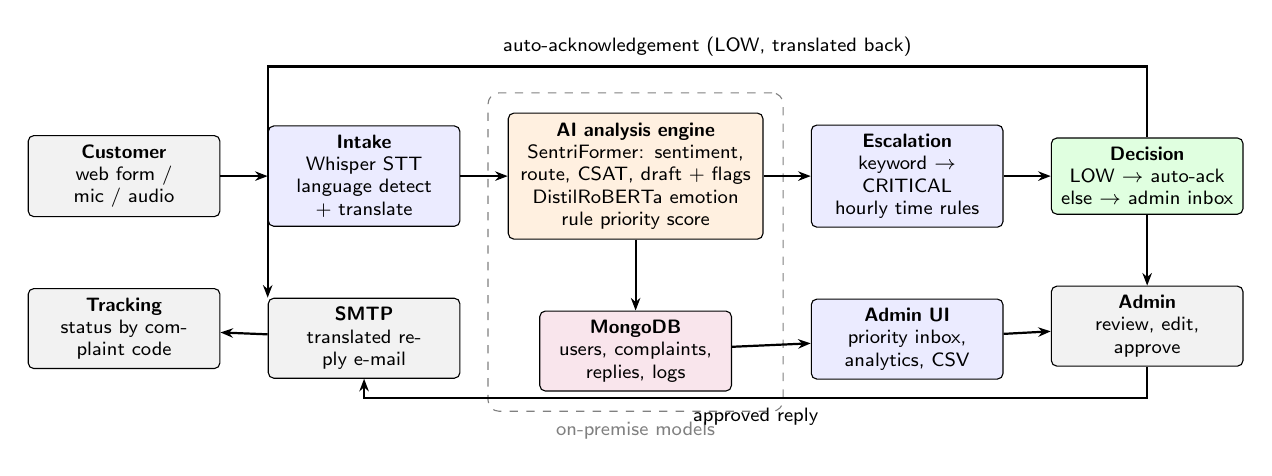
\begin{tikzpicture}[font=\sffamily\scriptsize, node distance=4mm and 6mm,
 b/.style={draw, rounded corners=2pt, align=center, minimum height=9mm, text width=2.2cm, fill=#1}, b/.default=white,
 ar/.style={-{Stealth[length=1.6mm]}, thick}, grp/.style={draw, dashed, rounded corners=4pt, inner sep=2.5mm, gray}]
\node[b=gray!10] (cust) {\textbf{Customer}\\ web form / mic / audio};
\node[b=blue!8, right=of cust] (intake) {\textbf{Intake}\\ Whisper STT\\ language detect + translate};
\node[b=orange!12, right=of intake, text width=3.0cm, minimum height=16mm] (ai) {\textbf{AI analysis engine}\\ SentriFormer: sentiment, route, CSAT, draft + flags\\ DistilRoBERTa emotion\\ rule priority score};
\node[b=blue!8, right=of ai] (esc) {\textbf{Escalation}\\ keyword $\rightarrow$ CRITICAL\\ hourly time rules};
\node[b=green!12, right=of esc] (dec) {\textbf{Decision}\\ LOW $\rightarrow$ auto-ack\\ else $\rightarrow$ admin inbox};
\node[b=gray!10, below=9mm of dec] (admin) {\textbf{Admin}\\ review, edit, approve};
\node[b=purple!10, below=9mm of ai] (db) {\textbf{MongoDB}\\ users, complaints, replies, logs};
\node[b=blue!8, below=9mm of esc] (ui) {\textbf{Admin UI}\\ priority inbox, analytics, CSV};
\node[b=gray!10, below=9mm of intake] (smtp) {\textbf{SMTP}\\ translated reply e-mail};
\node[b=gray!10, below=9mm of cust] (track) {\textbf{Tracking}\\ status by complaint code};
\draw[ar] (cust)--(intake); \draw[ar] (intake)--(ai); \draw[ar] (ai)--(esc); \draw[ar] (esc)--(dec);
\draw[ar] (dec)--(admin); \draw[ar] (ai)--(db); \draw[ar] (db)--(ui); \draw[ar] (ui)--(admin);
\draw[ar] (admin.south)--++(0,-4mm)-|node[pos=.25,below]{approved reply}(smtp.south);
\draw[ar] (smtp)--(track); \draw[ar] (dec.north)--++(0,9mm)-|node[pos=.25,above]{auto-acknowledgement (LOW, translated back)}(smtp.north west);
\begin{scope}[on background layer]\node[grp, fit=(ai)(db), label={[gray]below:on-premise models}] {};\end{scope}
\end{tikzpicture}}
\caption{SentriMail architecture. All models run locally. Model-generated drafts reach the customer only after administrator approval; automatic acknowledgements are limited to LOW-priority complaints.}
\label{fig:arch}
\end{figure*}

\section{Problem Definition and Research Gap}
Given a stream of complaints $\{x_i\}$ written in any of several languages, the system must (a) obtain an English text $\tilde{x}_i$, (b) assign a priority $p_i\in\{\text{LOW},\text{MEDIUM},\text{HIGH},\text{CRITICAL}\}$, (c) close low-risk complaints with an acknowledgement, and (d) give an administrator the evidence and a draft for the rest. It must do this on commodity hardware without external LLM APIs, and must never send model-generated text for complaints that need judgement.

Existing work covers pieces of this: routing, complaint detection, chatbots. Few published systems combine multilingual voice intake, explainable prioritisation and on-premise generative assistance with an explicit policy for which model outputs may affect customers. SentriMail is built to fill that gap.

\section{System Architecture}
Fig.~\ref{fig:arch} shows the components and Table~\ref{tab:stack} the technology stack.


\begin{table}[!t]
\centering
\caption{SentriMail implementation stack}
\label{tab:stack}
\footnotesize
\resizebox{\columnwidth}{!}{%
\begin{tabular}{@{}ll@{}}
\toprule
Layer & Technology (as implemented) \\
\midrule
Web backend & FastAPI 0.111 on uvicorn, 22 HTTP endpoints \\
Views & Jinja2 templates, Chart.js dashboards \\
Storage & MongoDB (pymongo 4.8): users, complaints, replies, login logs \\
Sessions / roles & HTTP-only cookie sessions; roles \texttt{user}, \texttt{admin} \\
Intake & web form, browser speech-to-text, Whisper (base) audio upload \\
Language & langdetect + machine translation (11 UI languages) \\
Models & SentriFormer (routing, sentiment, CSAT, draft reply); \\
 & DistilRoBERTa emotion; DistilBERT-SST2 / flan-T5-small fallbacks \\
Scheduling & APScheduler hourly time-based escalation \\
Notification & SMTP e-mail (outbound) \\
Deployment & Procfile, Python 3.11, PORT env var \\
\bottomrule
\end{tabular}}
\end{table}


\subsection{Intake and language handling}
Customers register, log in and submit a title and description through a web form. They can type, dictate with the browser's speech-recognition API, or upload an audio file that the server transcribes with Whisper (base model). If no language is supplied, it is detected and the text is translated to English for analysis. Both the original and translated text are stored, and every reply is translated back into the customer's language before delivery. Each complaint receives a human-readable code (\texttt{SENT-<year>-NNNN}) that anyone can use to track its status without logging in.

\subsection{AI analysis engine}
\texttt{analyze\_complaint()} orchestrates the models (Fig.~\ref{fig:flow}).

\textbf{SentriFormer.} The companion model is loaded once per process. One call returns a routing distribution over 33 product and issue categories, with a \emph{needs-triage} flag when the top probability is below 0.25. It also returns a 3-class sentiment, a 1--5 star satisfaction prediction, and a greedy-decoded draft reply. The draft is checked for repetition, template placeholders, invented URLs or contacts, unsupported names and orphaned channel phrases. Table~\ref{tab:model} summarises the offline evidence for these signals.

\textbf{Emotion.} A DistilRoBERTa emotion classifier gives one of seven emotions and its confidence.

\textbf{Priority score.} Sentiment and emotion are combined by an explicit rule so that every priority can be explained:
\begin{equation}
s = 40\,\sigma\,[\text{neg}] + 10\,[\text{neu}] + \lambda(e)\,\epsilon + 20\,[\text{trigger}] + 5\,[|x|>100],
\end{equation}
where $\sigma$ is the sentiment confidence and $\epsilon$ the emotion confidence; $\lambda(e)=40$ for anger, fear and disgust, 20 for sadness and surprise, and 0 otherwise. The trigger indicator fires on 18 urgency phrases, and $|x|$ is the word count. Scores of at least 75, 50 and 25 map to CRITICAL, HIGH and MEDIUM; lower scores map to LOW. A separate list of 11 safety keywords (e.g., legal, police, harassment) forces CRITICAL.

\textbf{Graceful degradation.} If SentriFormer cannot be loaded, sentiment falls back to DistilBERT-SST2 and then to a keyword lexicon. Emotion falls back to keyword patterns. The application keeps working with reduced capability.

\begin{figure}[!t]
\centering
\resizebox{!}{0.34\textheight}{%
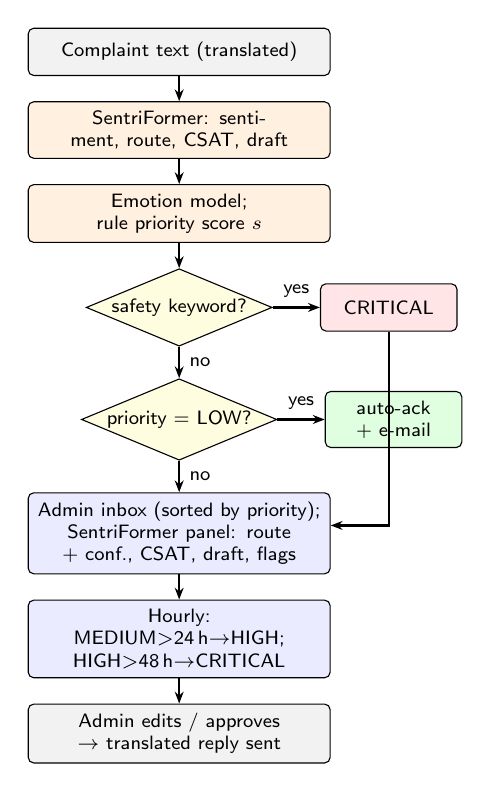
\begin{tikzpicture}[font=\sffamily\scriptsize, node distance=3.2mm,
 s/.style={draw, rounded corners=2pt, align=center, text width=3.6cm, minimum height=6mm, fill=#1}, s/.default=white,
 d/.style={draw, diamond, aspect=2.4, align=center, inner sep=0.5pt, fill=yellow!12},
 ar/.style={-{Stealth[length=1.5mm]}, thick}]
\node[s=gray!10] (a) {Complaint text (translated)};
\node[s=orange!12, below=of a] (b) {SentriFormer: sentiment, route, CSAT, draft};
\node[s=orange!12, below=of b] (c) {Emotion model; rule priority score $s$};
\node[d, below=of c] (d) {safety keyword?};
\node[s=red!10, right=6mm of d, text width=1.5cm] (crit) {CRITICAL};
\node[d, below=4mm of d] (e) {priority = LOW?};
\node[s=green!12, right=6mm of e, text width=1.5cm] (auto) {auto-ack + e-mail};
\node[s=blue!8, below=4mm of e] (f) {Admin inbox (sorted by priority); SentriFormer panel: route + conf., CSAT, draft, flags};
\node[s=blue!8, below=of f] (g) {Hourly: MEDIUM$>$24\,h$\rightarrow$HIGH; HIGH$>$48\,h$\rightarrow$CRITICAL};
\node[s=gray!10, below=of g] (h) {Admin edits / approves $\rightarrow$ translated reply sent};
\draw[ar] (a)--(b); \draw[ar] (b)--(c); \draw[ar] (c)--(d); \draw[ar] (d)--node[above]{yes}(crit); \draw[ar] (d)--node[right]{no}(e);
\draw[ar] (e)--node[above]{yes}(auto); \draw[ar] (e)--node[right]{no}(f); \draw[ar] (f)--(g); \draw[ar] (g)--(h);
\draw[ar] (crit.south)|-($(f.east)+(0,1mm)$);
\end{tikzpicture}}
\caption{Per-complaint workflow. Generated drafts appear only in the admin panel.}
\label{fig:flow}
\end{figure}

\subsection{Decision policy and human oversight}
Complaints whose final priority is LOW receive an automatic, translated acknowledgement by e-mail and are marked \emph{auto-replied}. All others are marked \emph{pending admin} and appear in an inbox sorted CRITICAL$>$HIGH$>$MEDIUM$>$LOW. An hourly scheduler escalates MEDIUM complaints pending for more than 24\,h to HIGH, and HIGH complaints pending for more than 48\,h to CRITICAL, so that nothing waits indefinitely. The admin's complaint page shows the sentiment and emotion meters, the priority and its description, and a suggested reply from priority-aware templates. A separate SentriFormer panel shows the routing category with its confidence (low-confidence routes are marked \emph{check manually}), the predicted CSAT and the generated draft with any raised flags. The draft is never pre-filled or sent automatically. The urgency output of SentriFormer is ignored by design, because it failed validation in the model study.

\subsection{Data, administration and analytics}
MongoDB stores users (hashed passwords, roles), complaints (original and translated text, all analysis fields, a SentriFormer sub-document, status and timestamps), replies and login logs, with indexes on user, status and creation time. The dashboard (Fig.~\ref{fig:ui}) shows totals, pending counts, resolutions today, average response time, and four charts: category, priority, daily volume and sentiment by category. Complaints can be exported to CSV.

\begin{figure}[!t]
\centering
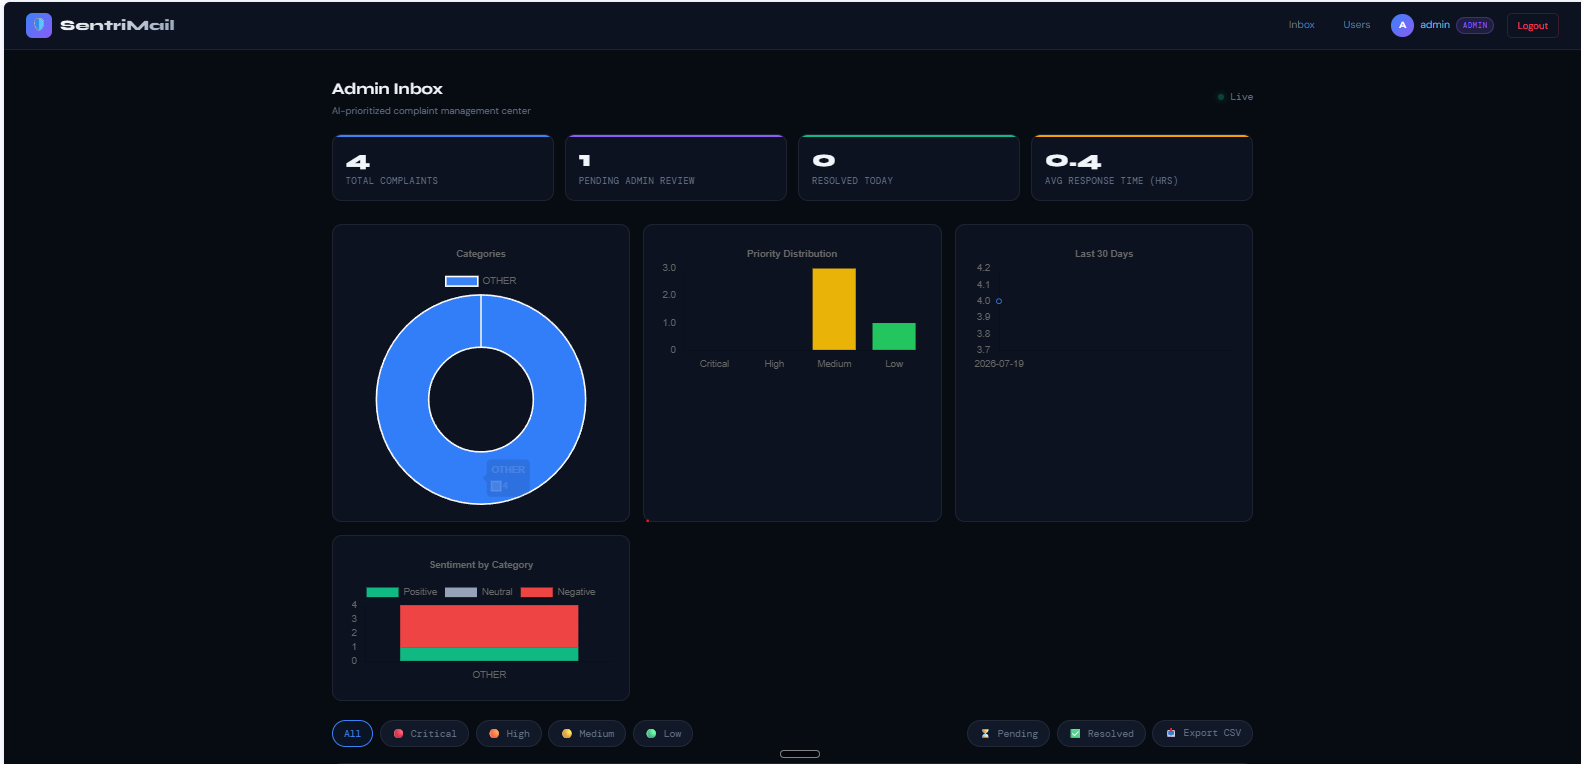
\includegraphics[width=\columnwidth]{admin_dashboard}\\[1mm]
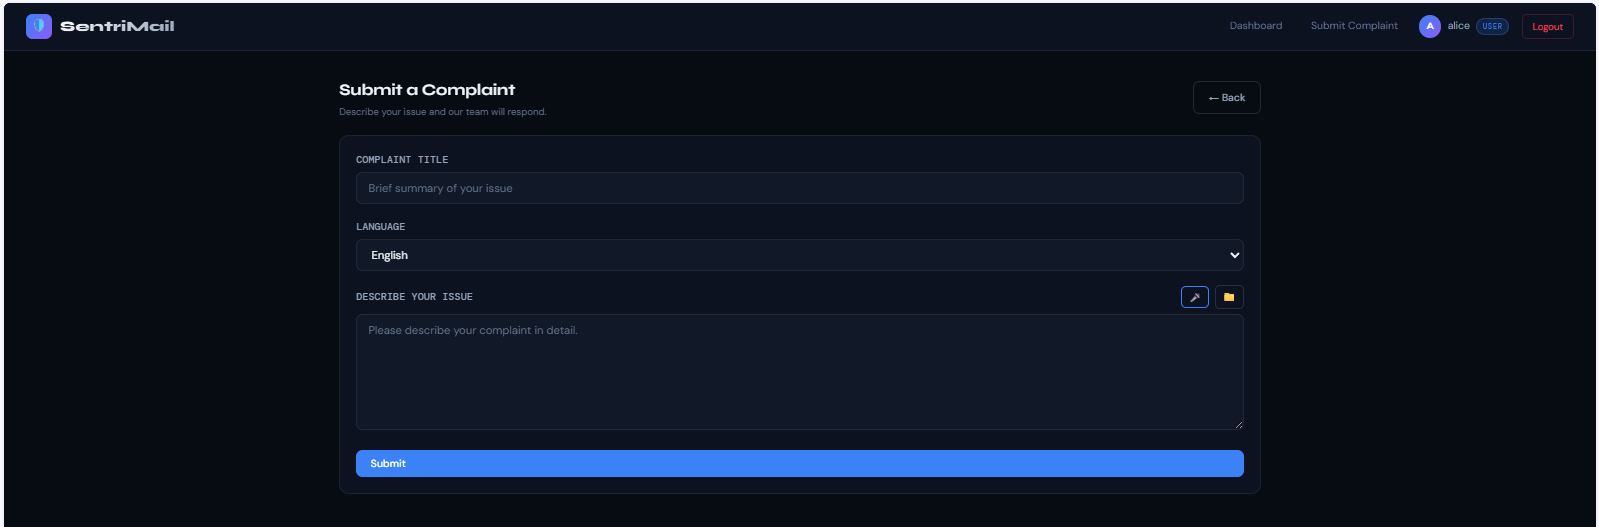
\includegraphics[width=0.85\columnwidth]{submit_form}
\caption{SentriMail user interface: admin inbox with KPIs and analytics (top); complaint submission with language selection, microphone and audio upload (bottom).}
\label{fig:ui}
\end{figure}

\begin{table}[t]
\centering
\caption{Offline quality of the SentriFormer signals consumed by SentriMail (held-out corpus splits, reported in the companion model study)}
\label{tab:model}
\footnotesize
\resizebox{\columnwidth}{!}{%
\begin{tabular}{@{}llr@{}}
\toprule
Signal used by SentriMail & Metric & Value \\
\midrule
Routing (33 classes, $n$=123{,}229, test) & accuracy / weighted-F1 & 73.7\% / 0.737 \\
 & majority baseline & 27.2\% \\
 & low-confidence ($<$0.25) rate & 0.5\% \\
Sentiment (3 classes, $n$=20{,}453, test) & accuracy / macro-F1 & 88.1\% / 0.758 \\
CSAT (1--5 stars, $n$=870, test) & exact / within-1 star & 72.4\% / 82.0\% \\
Draft reply (500 val.\ contexts, deployed) & broken-link / generic phrase & 0.4\% / 16.6\% \\
 & portal-loop & 1.0\% \\
Urgency & -- & not used (unvalidated) \\
\bottomrule
\end{tabular}}
\end{table}


\FloatBarrier
\section{Implementation and Experimental Setup}
SentriMail is implemented in Python (FastAPI, Jinja2, pymongo, APScheduler, Hugging Face Transformers, PyTorch). SentriFormer is imported from its own repository through a configurable path, so the application and the model can be versioned separately. The model is the deployed T5a checkpoint (46.7\,MB) described in the companion paper.

\textbf{Latency benchmark.} We wrote a benchmark set of 30 complaint messages (4--58 words) covering billing, delivery, account access, fraud, lending, mortgages, service quality and positive feedback. Each model stage was timed in isolation with two repetitions per message after a warm-up call (flan-T5 once per message), on an RTX~3060 Laptop GPU and on the laptop CPU with 8 PyTorch threads. We also ran the integrated \texttt{analyze\_complaint()} function on all 30 messages, replicating the application's post-analysis keyword escalation and LOW-priority branch, to record end-to-end latency and the resulting decisions. No database or web server was involved in these measurements.

\FloatBarrier
\section{Results and Discussion}
\subsection{Latency}
Table~\ref{tab:lat} and Fig.~\ref{fig:lat} report the measurements. All SentriFormer heads together take a median of 30\,ms on the CPU. That is faster than the DistilBERT sentiment model alone (42\,ms), even though SentriFormer also produces routing and CSAT. Adding the generated draft brings the total to 275\,ms. The sampled flan-T5-small reply used by the previous version of the application is about 3$\times$ slower (844\,ms median) and has a heavy tail (p95 3.1\,s). At batch size one, the CPU beats the GPU for SentriFormer because kernel-launch overhead dominates a model this small; the larger DistilBERT models gain from the GPU. The integrated analysis of a complaint takes 531\,ms median (p95 649\,ms). The first call, which loads every model, takes 43\,s and happens once per process.

\begin{table}[t]
\centering
\caption{Measured per-stage inference latency (ms; 30 messages $\times$ 2 repetitions; flan-T5 $\times$ 1)}
\label{tab:lat}
\footnotesize
\resizebox{\columnwidth}{!}{%
\begin{tabular}{@{}lrrrr@{}}
\toprule
 & \multicolumn{2}{c}{CPU (8 threads)} & \multicolumn{2}{c}{GPU (RTX 3060 6\,GB)} \\
\cmidrule(lr){2-3}\cmidrule(l){4-5}
Stage & median & p95 & median & p95 \\
\midrule
SentriFormer heads (route, sentiment, CSAT) & \textbf{30.4} & 33.9 & 59.4 & 65.7 \\
SentriFormer heads + draft reply (greedy) & 275.2 & 501.8 & 586.0 & 898.1 \\
DistilBERT-SST2 sentiment (fallback) & 41.9 & 51.7 & 19.6 & 23.4 \\
DistilRoBERTa emotion & 37.8 & 51.9 & 20.8 & 24.7 \\
flan-T5-small auto-reply (sampled) & 843.6 & 3095.9 & 1690.1 & 4345.1 \\
SentriFormer checkpoint load & \multicolumn{2}{c}{720.7 (once)} & \multicolumn{2}{c}{1095.0 (once)} \\
\midrule
Full \texttt{analyze\_complaint()} (integrated) & -- & -- & 531.1 & 649.3 \\
\bottomrule
\end{tabular}}
\end{table}


\begin{figure}[!t]
\centering
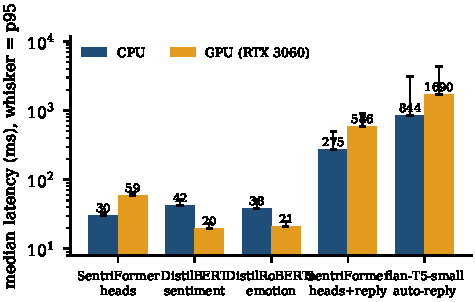
\includegraphics[width=\columnwidth]{latency}
\caption{Median per-stage inference latency (log scale; whiskers show p95).}
\label{fig:lat}
\end{figure}

\subsection{Pipeline behaviour}
Table~\ref{tab:pipe} summarises the decisions on the benchmark. SentriFormer output was attached to every complaint. Only the two thank-you messages were classified LOW and auto-acknowledged; no message containing a refund, fraud or legal term was auto-replied. The two CRITICAL cases were an identity-theft report and a foreclosure notice, both of which a human would escalate. Five complaints (17\%) were routed with confidence below 0.25 and flagged for manual checking. That is much higher than the 0.5\% rate on the CFPB test split, because the benchmark includes e-commerce and service messages, which are rare in the routing training data. No reply-safety flag was raised on any of the 30 drafts. These numbers show that the system behaves as intended on representative input; they are not an accuracy estimate.

\begin{table}[!t]
\centering
\caption{Integrated pipeline decisions on the 30-message benchmark}
\label{tab:pipe}
\footnotesize
\resizebox{\columnwidth}{!}{%
\begin{tabular}{@{}lr@{}}
\toprule
Quantity & Value \\
\midrule
Messages with SentriFormer output attached & 30 / 30 \\
Final priority: CRITICAL / HIGH / MEDIUM / LOW & 2 / 16 / 10 / 2 \\
Auto-replied (LOW) & 2 (both thank-you messages) \\
Auto-replied while containing a hard-blocker term & 0 \\
Routing flagged for manual triage (conf.\ $<$0.25) & 5 / 30 \\
Draft replies with a safety flag raised & 0 / 30 \\
Sentiment: negative / positive & 28 / 2 \\
Predicted CSAT stars 1/2/3/4/5 & 6 / 5 / 7 / 3 / 9 \\
First call incl.\ model loading & 43.2\,s \\
\bottomrule
\end{tabular}}
\end{table}


\subsection{Discussion}
The design choices follow from the evidence. Sentiment, which is well supported offline (88.1\% accuracy), is the only SentriFormer output that changes system behaviour. Routing (73.7\% over 33 classes) is shown with its confidence and a manual-check flag, in line with confidence-gated routing practice~\cite{mandal2018cognitive}. CSAT, whose minority classes are poorly predicted, is shown only as a hint. Drafts remain suggestions because ROUGE-based and rule-based reply metrics cannot certify correctness~\cite{ji2023survey}. The rule-based priority layer keeps every decision explainable in terms an administrator can check, and the hourly escalation bounds the waiting time of any complaint.

\FloatBarrier
\section{Limitations and Future Scope}
\textbf{Evaluation.} SentriMail has not yet been evaluated with real users. A labelled set of priority decisions, measurements of admin acceptance and edit distance for drafts, and a usability study are needed to quantify its benefit. The latency measurements cover model inference, not translation or e-mail delivery.
\textbf{Decision boundaries.} Our audit of the code found that the auto-acknowledgement branch checks only the LOW priority. A stricter auto-resolvability test, which blocks refund, chargeback, legal, fraud and similar terms and very negative sentiment, is computed but not enforced; enforcing it is a one-line change. Routing output is advisory and not yet used to assign complaints to teams, and the stored category field is not populated from it.
\textbf{Engineering.} The admin page re-runs the full analysis, including generation, on each view; caching the stored SentriFormer result would remove this cost. Sessions are held in process memory and passwords use unsalted hashing; production deployment needs persistent sessions, salted key-derivation, CSRF protection and authentication on the transcription endpoint. The JSON fallback store does not support every query the application uses, so MongoDB is required.
\textbf{Future work.} Retrieval-augmented drafts grounded in policy documents~\cite{lewis2020rag}, using admin edits as a training signal~\cite{zhao2025agent}, mapping the 33 routing classes to organisational teams, inbound e-mail ingestion, and a validated urgency model.

\section{Conclusion}
SentriMail shows how a compact on-premise language model can be integrated into a complaint-management workflow responsibly. Each model output is used only where its offline evidence supports it, every priority decision is explainable, and generated text reaches customers only after human approval. With multilingual and voice intake, hybrid prioritisation, time-based escalation and analytics, the system analyses a complaint in about half a second on a laptop. The next step is a user study to measure its effect on response time and resolution quality.

\section*{Acknowledgment}
The authors thank Prof.\ Syeeda Mujeebunnisa for her guidance and BMS College of Engineering, Bengaluru, for providing the facilities used in this work.

\balance
\bibliographystyle{IEEEtran}
\bibliography{references}

\end{document}
